\documentclass[xcolor=svgnames,handout]{beamer}
\usepackage{alltt}
\usepackage{graphicx}
\usepackage[utf8]{inputenc}
\usepackage{pifont}  % checkmark sybmols
\usepackage{xspace}

\graphicspath{{figs/}}

\usetheme{bro}

\title{Bro Live!: Training for the Future}
%\subtitle{Bro Workshop 2011}
\author{Jon Schipp\\
\small NCSA\\
\texttt{jschipp@illinois.edu}}
\institute{%
BroCon14\\
NCSA, Champaign-Urbana, IL
}
%\date[]{\footnotesize November 9, 2011}
\date[]{}

\newcommand{\checked}{\textcolor{olive}{\ding{51}}\xspace}
\newcommand{\unchecked}{\textcolor{red}{\ding{55}}\xspace}

\begin{document}

\begin{frame}[plain]
  \titlepage
\end{frame}

\section{Motivations}

\begin{frame}[fragile]{Motivations}
  \begin{block}{Issues}
    \begin{itemize}
      \item \textcolor{red}{Users:} Too much time is spent passing around, downloading, and copying Virtual Machines or other materials
    	\begin{itemize}
		\item Networks are slow
		\item Virtual harddisks are big
    	\end{itemize}
      \item \textcolor{red}{Users:} Technical difficulties can occur and often do that end up putting some behind the group
    	\begin{itemize}
      		\item VirtualBox bus configuration
      		\item VirtualBox network configuration
    	\end{itemize}
      \item \textcolor{red}{Admins:} Account management is repetitive
      \item \textcolor{red}{Everyone:} Changes are not easy
    	\begin{itemize}
      		\item Insertion of wrong exercises, mistakes, etc.. How is this handled?
    	\end{itemize}
    \end{itemize}
  \end{block}
 \begin{center}
    \item[$\Rightarrow$]
      \alert{Ultimately, the burden is placed on the users and this affects the overall event experience}
  \end{center}
\end{frame}

\begin{frame}{Solutions}
  \begin{block}{Ideas}
    \begin{itemize}
      \item \textcolor{red}{Admins:} Avoid passing around or downloading VM’s if possible. Give user’s access to your server. Big time saver!
      \item \textcolor{red}{Admins:} Make barrier to participation as thin as possible
    	\begin{itemize}
		\item Require only a program (e.g. ssh)
		\item Opens possibilities to phones, tablets, etc.
    	\end{itemize}
      \item \textcolor{red}{Admins:} Automated account management
      \item \textcolor{red}{Admins:} Changes can be easily completed
    	\begin{itemize}
		\item Add, remove, or modify exercises during event
		\item Immediately available
    	\end{itemize}
    \end{itemize}
  \end{block}
 \begin{center}
    \item[$\Rightarrow$]
      \alert{Ultimately, we pass the burden onto the admins (we’re used to it anyway)}
  \end{center}
\end{frame}

\begin{frame}{Major Software Components}
  \begin{center}
    
\includegraphics[width=.8\textheight]{components.png}
  \end{center}
  \begin{center}
    \fbox{You know at least four of these right?}
  \end{center}
\end{frame}

\begin{frame}{Docker}
  \begin{block}{What?}
  \begin{itemize}
      \item Automates the deployment of Linux based containers
      \item Provides a layer of abstraction
      \item Various methods of container creation
  \end{itemize}
  \end{block}
  \begin{center}
    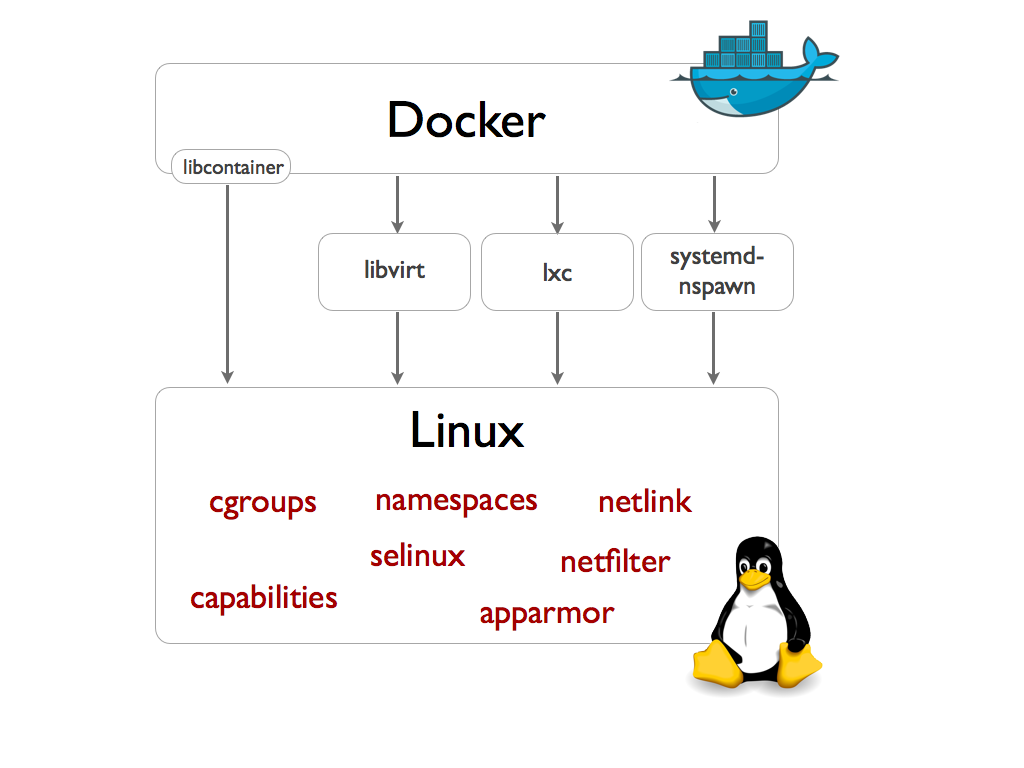
\includegraphics[width=.7\textwidth]{docker-abstraction.png}
  \end{center}
\end{frame}

\begin{frame}{Linux Based Containers}
  \begin{itemize}
    \item \textbf{Important:} "Linux \textit{Based} Containers"
      \begin{itemize}
        \item There is no container specification
        \item There are different container (and like) technologies for Linux
      	\begin{itemize}
        	\item \textbf{Linux:} LXC, OpenVZ,  Google containers, etc.
        	\item \textbf{Non-Linux:} BSD Jails, Solaris Zones, AIX WPAR, etc.
      	\end{itemize}
      \end{itemize}
    \item \textbf{What} do containers do?
      \begin{itemize}
        \item Light-weight process virtualization
      \end{itemize}
    \item \textbf{What} do virtual machines do?
      \begin{itemize}
        \item Hardware virtualization
      \end{itemize}
  \end{itemize}
\end{frame}

\begin{frame}{Linux Kernel Stuff}
  \begin{itemize}
    \item \textbf{Support:} Linux Kernel 3.8 introduced the foundation for Linux Based containers
      \begin{itemize}
        \item Namespaces
      		\begin{itemize}
        		\item Currently available: \textit{pid, net, ipc, uts, mnt, and user}
        		\item Process isolation
      		\end{itemize}
        \item Control Groups (cgroups)
      		\begin{itemize}
        		\item Resource Management
      		\end{itemize}
      \end{itemize}
    \item \textbf{It’s not magic}, you can create namespaces and cgroups directly from your shell by modifying procfs and sysfs
  \end{itemize}
\end{frame}


\begin{frame}{Container Advantages}
  \begin{itemize}
    \item \textbf{Density:} Run hundreds or even thousands of containers on a single machine
    \item \textbf{Performance:} Very fast startup and tear down time, little overhead
    \item \textbf{Nesting:} Running containers within containers is possible
    \item \textbf{Isolation:} See or talk to hosts, other containers, or none
    \item \textbf{User Perspective:} Looks and feels like a Virtual Machine
	\begin{itemize}
       		\item Container has its own IP, filesystem, processes, etc.
      	\end{itemize}
  \end{itemize}
\end{frame}

\begin{frame}{Our Implementation}
  \begin{enumerate}
    \item Users log into a non-privileged system account via SSH
  	\begin{itemize}
		\item Strong crypto, ubiquitious, low overhead
		\item ssh demo@live.bro.org
	\end{itemize}
    \item Automated account (non-system) creation via shell script
    \item Docker is called and ships each user in their own container
  	\begin{itemize}
		\item Appropriately named and thus re-attachable by name
		\item Handled via shell script
		\item \textcolor{red}{Just in case you forgot each container instance is an isolated process}
	\end{itemize}
    \item User performs work in container
  	\begin{itemize}
		\item Runs unix commands, traverses filesystem, runs bro
	\end{itemize}
    \item User logs out, does something else then is ready to work again
  	\begin{enumerate}
		\item They SSH into the same non-privileged user account again
	 	\item Enter their newly created credentials
	 	\item Are automatically re-attached to their container instance
	\end{enumerate}
  \end{enumerate}
\end{frame}

\begin{frame}{Container Security Considerations}
  \begin{itemize}
    \item Networking is disabled
	\begin{itemize}
		\item Prevent attacks against other hosts, containers, or self
	\end{itemize}
    \item System resources are limited per container to prevent selfishness and abuse
	\begin{itemize}
		\item CPU and RAM allocation
	\end{itemize}
    \item Containers and users are automatically removed after a period of time
	\begin{itemize}
		\item Length of conference or event
	\end{itemize}
    \item Containers which get too large are automatically removed to prevent disk space abuse
	\begin{itemize}
		\item Denial of Service
	\end{itemize}
    \item Finer environment controls via ulimit
	\begin{itemize}
		\item fsize, nproc, etc.
	\end{itemize}
  \end{itemize}
\end{frame}


\begin{frame}{Want Your Own?}
  \begin{block}{You too can have one too}
    \begin{itemize}
      \item Want to host your own Bro training event with a system like this?
    	\begin{itemize}
		\item It's free
		\item Publicly available
		\begin{itemize}
			\item \textbf{Vagrant:} http://github.com/jonschipp/vagrant
			\item \textbf{Docker:} http://hub.docker.com/u/jonschipp/latest-bro-sandbox/
		\end{itemize}
		\item System configuration is entirely automated
	\end{itemize}
	\item Written for and tested on Ubuntu Trusty and Saucy
    \end{itemize}
  \end{block}
  \begin{exampleblock}{Installation and configuration on Ubuntu}
	\alert{\$ wget https://raw.githubusercontent.com/jonschipp/vagrant/
	master/bro-sandbox/provision.sh -O - | bash}
  \end{exampleblock}
  \begin{exampleblock}{Testing with Vagrant}
	\alert{\$ git clone http://github.com/jonschipp/vagrant \&\& cd vagrant/bro-sandbox \&\& vagrant up; ssh -p 2222 demo@127.0.0.1}
  \end{exampleblock}
\end{frame}

\begin{frame}{Demo}
  \begin{exampleblock}{Let's try it}
\begin{semiverbatim}
\$ ssh demo@live.bro.org \newline
demo@live.bro.org's password:  \newline
Welcome to Bro Live! \newline
==================== \newline
... 		     \newline
A place to try out Bro. \newline
Are you a new or existing user? [new/existing]: new \newline
... \newline
Enjoy yourself! \newline
Training materials are located in /exercises. \newline
e.g. \$ bro -r /exercises/BroCon14/beginner/http.pcap \newline
demo@bro:~\$
\end{semiverbatim}
  \end{exampleblock}
\end{frame}

\begin{frame}{Feedback}
  \begin{itemize}
    \item \textbf{Beta:} The beta is live today!
    	\begin{itemize}
		\item Help me help you
 	\item Report any problems or concerns with usability or security
    	\item Send me feature requests
	        \item Send me patches and pull requests
  	\end{itemize}
  \end{itemize}
  \begin{exampleblock}{Let me know}
  \textcolor{red}{Talk to me} \newline
  \textcolor{blue}{Tweet  me:} @JonSchipp \newline
  \textcolor{blue}{E-mail me:} jonschipp@gmail.com, jschipp@illinois.edu \newline
  \end{exampleblock}
\end{frame}

\begin{frame}[allowframebreaks]{References}
\begin{thebibliography}{1}
\bibitem[SP10]{Rosen}
Rami Rosen
\newblock {Resource management: Linux kernel Namespaces and cgroups}.
\newblock In {\em http://www.haifux.org/lectures/299/netLec7.pdf}

\bibitem[KMV{\etalchar{+}}14]{Rosen}
Rami Rosen
\newblock {Linux Containers and the Future Cloud}.
\newblock In {\em http://www.haifux.org/lectures/320/netLec8\_final.pdf}

\bibitem[SP10]{Petazonni}
Jerome Petazzoni
\newblock {Lightweight Virtualization with Linux Containers (LXC)}.
\newblock In {\em http://www.ciecloud.org/2013/subject/07-track06-Jerome\%20Petazzoni.pdf} The 5th China Cloud Computing Conference, China National Convention Center, Beijing

\bibitem[SP10]{Docker}
Docker
\newblock {\em www.docker.com}

\end{thebibliography}
\end{frame}

\end{document}
